\section{Method}
To evaluate the performance of Reinforcement Learning and Genetic Algorithms,
experiments have been conducted on the simple but effective environment of the cart pole.

Cart Pole is a classic control problem in reinforcement learning. 
The goal is to balance a pole on a cart that can move left or right. 

The state space is four-dimensional, consisting of the cart position, cart velocity, pole angle, and pole angular velocity $[p, v, \alpha, \omega]$. 

The action space is discrete, with two possible actions: move left or move right. 

The reward is 1 for every time step the pole is balanced.

The goal is to balance the pole for as long as possible, with a limit of 500 actions.

The environment, called \textit{CartPole-v1}, is implemented in Python using the Gymnasium library \cite{towers_gymnasium_2023}.
\\
Below described implementations have been trained using the same enviromnemt and ensuring that in every iteration the starting point is the same between two methods, but different from the previous iteration, to ensure that the comparison can be evaluated \textcolor{blue}{without considering the stochastic nature of the training}.

\subsection{Reinforcement Learning}
The reinforcement learning implementation is based on temporal differenc learning \cite{sutton1998temporal}, 
in particular Q-learning.
The implementation takes inspiration on the work of \textit{JackFurby} \cite{JackFurbyCartPole}.

The \textit{Q-table} is represented by the discretization of the continuous 4-dimensional state vector in 20 even intervals for every dimension of the vector leading to 160000 possible pairs of $<state,action>$, considering the two possible actions.

\begin{figure}[H]
	\centering
	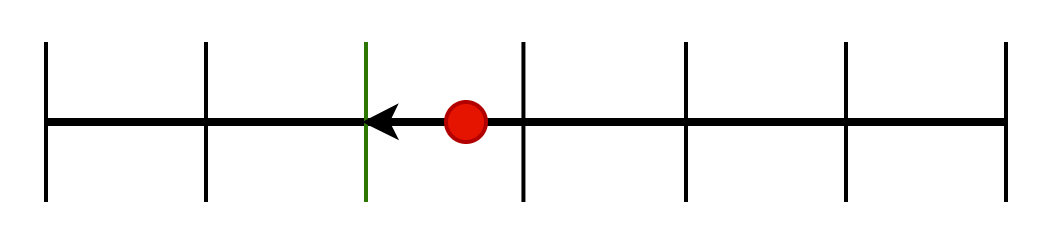
\includegraphics [scale = 0.2]{Images/state_discretization.png}
	\caption{Representation of the state discretization technique, considering an element of the 4D-state, $s_i$, the red dot is the real value of $s_i$, this is discretized to the nearest leftwise discrete state.}
	\label{figDISC}
\end{figure}

Once an action is performed, the state selected is the first larger that the observed state.\\
The parameters used in the experiments are the following:


\begin{table}[htb]%
	\centering
	\label{tab:RL_parameters}
	\begin{tabular}{|S|S|} 		% S = special column format from the siunitx package. Aligns commas.
		
		\hline
		{\textbf{Learning rate $\alpha$}} &  {0.1} \\
		\hline
		{\textbf{Discount factor $\gamma$}} & {1} \\
		\hline
		{\textbf{Number of episodes $n_{ep}$}} & {20000} \\
		\hline
		{\textbf{Exploration rate $\varepsilon$}}  & {variable} \\
		\hline
		{\textbf{Mutation Rate}} & {0.05} \\
		\hline
		{\textbf{Penalty factor $PF$}}& {-375} \\
		\hline
		
	\end{tabular}
	\caption{Parameters used in the RL implementation. The exploration rate $\varepsilon$ starts with $\varepsilon(0)=1$ and decays by $\varepsilon(t) = \varepsilon(t - 1) - \frac{1}{\frac{n_{ep}}{2} - 1}$, every episode, stopping after $\frac{n_{ep}}{2}$ episodes. }
\end{table}



\subsection{Genetic Algorithms}

\textbf{Genotype}\\
Since Genetic Algorithms can be very different depending on the genotype chosen to represent individuals, we have tried several different implementation of GA, varying the used genotype.
\\

\subsubsection{Encoding the sequence of actions}
The first method used is a very naive implementation that can be applied to a very large variety of problems with GA : reprensenting individuals with the vector of all actions they will perform in order.
Thus, \textit{i-th} character of the genotype of an individual $j$ corresponds to the \textit{i-th} action performed by the corresponding individual.
In this apporach, mutation is performed by switching an action in the genotype from left to right or from right to left with a probability given by the \textit{Mutation rate} for every action $i$ inside the genotype.
\\
Since this particular genotype does not generalize well with the random initialization of the starting position of the pole. Due its intrinisc dependecy with the initial state, fixed starting conditions should be applied to effectively train in a meaningful way this genotype, by seeding the environment to always start in the same place, but this leads to a scarse ability of generalization, since the training is valid just for a determinated starting position of the pole.

All those considerations lead to the decision of evaluating other encodings for the final implementation.\\
\subsubsection{Encoding a state-action table}
The second encoding takes inspiration from Reinforcement Learning \textit{Q-table}.
In this approach, the focus is not to predict every action one by one  but instead use GA to assign values to state-actions pairs then select the action that referes to the observed state.\\
The discretization techninque is the same used in the reinforcement learning implementation and briefly described in figure \ref{figDISC}.\\
Here, mutation is performed by swapping the action of a given state with a probability given by the \textit{Mutation rate}.
\\

\textbf{Parameters}\\
The GA parameters can be found in the following table :
\begin{table}[htb]%
	\centering
	\caption{Parameters used in the GA implementation}
	\label{tab:GA_parameters}
	\begin{tabular}{|S|S|} 		% S = special column format from the siunitx package. Aligns commas.
		
		\hline
		{\textbf{Genotype}} &  {Q-table} \\
		\hline
		{\textbf{Population Size}} & {100} \\
		\hline
		{\textbf{Generations}} & {200} \\
		\hline
		{\textbf{Selection}}  & {Fitness} \\
		\hline
		{\textbf{Mutation Rate}} & {0.005} \\
		\hline
		{\textbf{Crossover}}& {one-point} \\
		\hline
		{\textbf{\textcolor{blue}{Elitism}}}& {\textcolor{blue}{2} } \\
		\hline

	\end{tabular}
\end{table}


